\documentclass{article}
\usepackage{iclr2025_conference,times}
\usepackage[utf8]{inputenc}
\usepackage[T1]{fontenc}
\usepackage{hyperref}
\usepackage{url}
\usepackage{booktabs}
\usepackage{amsmath,amsfonts}
\usepackage{graphicx}
\usepackage{subcaption}
\usepackage{tikz}
\usetikzlibrary{positioning,arrows.meta,shapes.geometric}

\title{Category-Guided Line Art Generation from Images}

\author{
YiYang Gao \\
University of Toronto \\
APS360 -- Winter 2026
}

\begin{document}
\maketitle

% ============================================================
\section{Brief Project Description}
% ============================================================

Given a photograph, our system classifies it into one of three categories---\textbf{biological} (animals/humans), \textbf{building}, or \textbf{vehicle}---then routes it to a category-specific U-Net [1] that generates a line art drawing in the appropriate style (Figure~\ref{fig:pipeline}).
Different subjects demand different line styles: animals need flowing organic curves, architecture needs straight geometric edges, and vehicles need clean mechanical contours.
Classical edge detectors [2] are category-agnostic and cannot capture these distinctions.
Deep learning lets us learn category-dependent features that separate salient contours from texture noise, and generate artistic line strokes rather than raw gradients.
Our two-stage design decomposes the problem into image classification and image-to-image translation---both well-suited to CNNs.

\begin{figure}[h]
\centering
\vspace{-2mm}
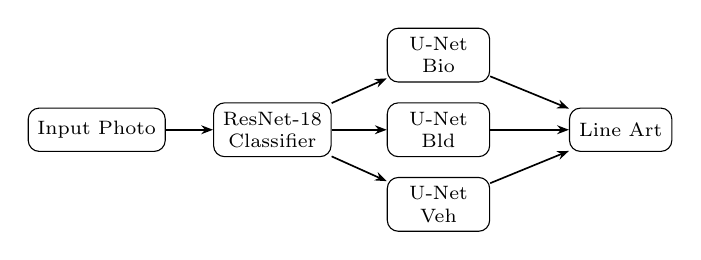
\begin{tikzpicture}[
  node distance=0.45cm and 0.6cm,
  box/.style={draw, rounded corners, minimum height=0.55cm, minimum width=1.3cm, font=\scriptsize, align=center},
  arrow/.style={-{Stealth[length=1.5mm]}, semithick}
]
  \node[box] (input) {Input Photo};
  \node[box, right=of input] (cls) {ResNet-18\\Classifier};
  \node[box, above right=0.25cm and 0.7cm of cls] (bio) {U-Net\\Bio};
  \node[box, right=0.7cm of cls] (bld) {U-Net\\Bld};
  \node[box, below right=0.25cm and 0.7cm of cls] (veh) {U-Net\\Veh};
  \node[box, right=1.0cm of bld] (out) {Line Art};
  \draw[arrow] (input) -- (cls);
  \draw[arrow] (cls) -- (bio);
  \draw[arrow] (cls) -- (bld);
  \draw[arrow] (cls) -- (veh);
  \draw[arrow] (bio) -- (out);
  \draw[arrow] (bld) -- (out);
  \draw[arrow] (veh) -- (out);
\end{tikzpicture}
\vspace{-2mm}
\caption{System pipeline: classifier routes the input to a category-specific U-Net for stylised line art generation.}
\label{fig:pipeline}
\vspace{-4mm}
\end{figure}

% ============================================================
\section{Notable Contribution}
% ============================================================

% ------ 2.1 DATA PROCESSING ------
\subsection{Data Processing}

\textbf{Classification data.}
We collected 2{,}000 images per category (6{,}000 total), split 70/15/15\% into train/val/test (Table~\ref{tab:data}).
Sources: iNaturalist 2021 [3] filtered to \texttt{kingdom=Animalia}; Places365 [4] (20 architecture scene categories); Stanford Cars via HuggingFace.
All images resized to $256{\times}256$; training uses random crop ($224{\times}224$), horizontal flip, colour jitter, and ImageNet normalisation.

\textbf{Line art data.}
We generate spatially-aligned (photo, line art) targets via multi-scale gradient edge detection (Sobel at $\sigma\in\{1,2,4\}$, percentile thresholding, morphological cleanup) applied to the classification images, producing the same 1{,}400/300/300 split per category.
Figure~\ref{fig:samples} shows representative training pairs.

\textbf{Testing plan.} We will collect $\sim$50 new photographs per category (self-captured or from unseen sources) for blind final evaluation.

\textbf{Challenges.}
(1)~iNaturalist contains plants/fungi; resolved by kingdom filtering.
(2)~Stanford Cars original download URL broken; used HuggingFace mirror.
(3)~We initially used Sketchy Database [5] human sketches as targets but found they are \emph{not spatially aligned} with photos, causing blurry U-Net outputs. We pivoted to edge-detection targets (see Section~\ref{sec:lineart_results}).

\begin{table}[h]
\centering
\vspace{-2mm}
\caption{Dataset statistics (identical split for classification and line art data).}
\label{tab:data}
\vspace{1mm}
\small
\begin{tabular}{llccc}
\toprule
\textbf{Category} & \textbf{Source} & \textbf{Train} & \textbf{Val} & \textbf{Test} \\
\midrule
Biological & iNaturalist 2021 (Animalia) & 1{,}400 & 300 & 300 \\
Building   & Places365 (20 scene types) & 1{,}400 & 300 & 300 \\
Vehicle    & Stanford Cars & 1{,}400 & 300 & 300 \\
\bottomrule
\end{tabular}
\vspace{-4mm}
\end{table}

\begin{figure}[h]
\centering
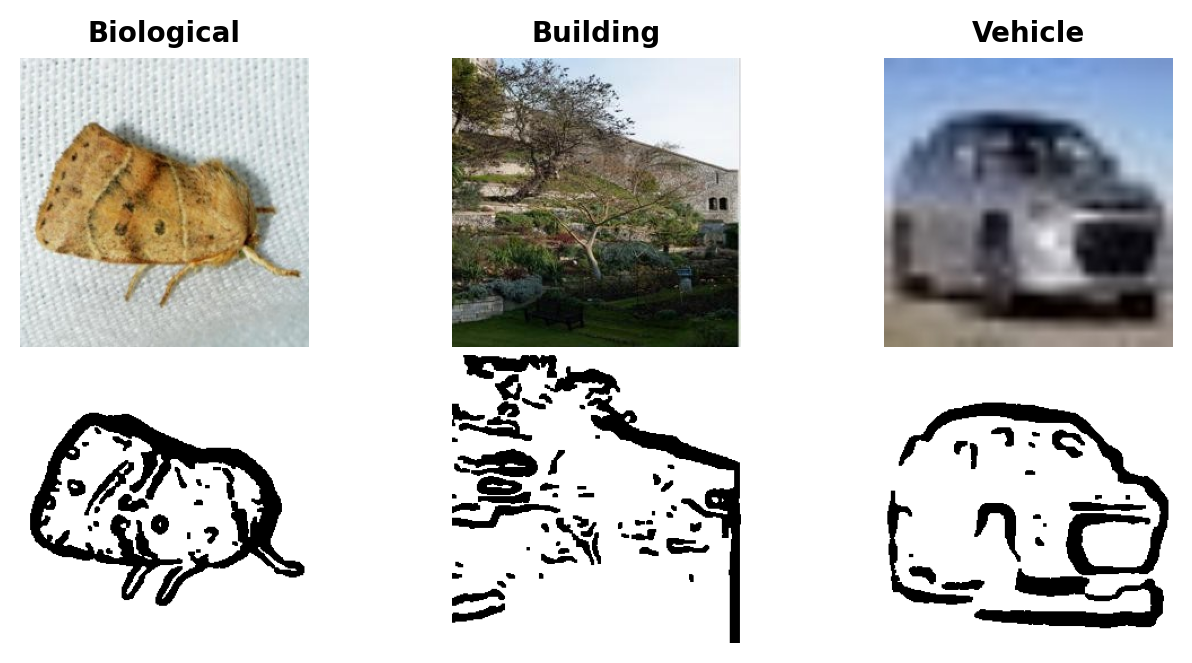
\includegraphics[width=0.75\textwidth]{figures/data_samples.png}
\vspace{-3mm}
\caption{Sample training pairs: input photos (top) and edge-detection line art targets (bottom).}
\label{fig:samples}
\vspace{-4mm}
\end{figure}

% ------ 2.2 BASELINE MODEL ------
\subsection{Baseline Model}

\textbf{Classification:} 3-layer CNN (Conv$3{\times}3$--ReLU--MaxPool $\times 3$, FC $\to 256 \to 3$ with dropout; $\sim$25M params). Trained with Adam ($\text{lr}{=}10^{-4}$), early stopping after 11 epochs.
\textbf{Line art:} Canny edge detection with fixed thresholds ($\text{low}{=}50$, $\text{high}{=}150$), category-agnostic; requires no learning and serves as a lower bound.

The baseline CNN achieves \textbf{84.56\%} test accuracy (Table~\ref{tab:results}).
Building is the weakest class (79.33\%), with 55 of 62 errors being buildings misclassified as biological, likely due to within-class diversity (e.g.\ gardens containing vegetation).
Vehicle is most separable (90.33\%).
Figure~\ref{fig:curves}a shows loss and accuracy curves; the model converges by epoch 8 with a visible train--val gap indicating limited capacity.

% ------ 2.3 PRIMARY MODEL ------
\subsection{Primary Model}

\textbf{Classifier:} ResNet-18 [6] pretrained on ImageNet ($\sim$11.2M params), final FC replaced with 3-class head. Fine-tuned end-to-end with Adam ($\text{lr}{=}10^{-4}$), batch size 32, early stopping at epoch 10.

\textbf{Generator:} Per-category U-Net ($\sim$7.8M params each). Encoder: 4 DoubleConv blocks (Conv$3{\times}3$--BN--ReLU $\times 2$, MaxPool) with channels $3{\to}32{\to}64{\to}128{\to}256$; bottleneck at 512; decoder mirrors encoder with transposed convolutions and skip connections; $1{\times}1$ conv + sigmoid output.
Input: $128{\times}128$ RGB; output: 1-channel line art.
Loss: weighted BCE ($w_{\text{fg}}{=}5$) + $L_1$ to address foreground sparsity ($<$10\% of pixels are lines).
Trained with Adam ($\text{lr}{=}2{\times}10^{-4}$), ReduceLROnPlateau, batch 16, up to 25 epochs.

\textbf{Classification results.}
ResNet-18 achieves \textbf{98.78\%} test accuracy ($+14.2$pp over baseline), with $>$97\% per-class (Table~\ref{tab:results}).
Only 11/900 test images are misclassified; 6 are buildings confused with biological.
Transfer learning from ImageNet is highly effective for this 3-class task (Figure~\ref{fig:curves}b).

\begin{table}[h]
\centering
\vspace{-2mm}
\caption{Classification test accuracy (300 images per class, 900 total).}
\label{tab:results}
\vspace{1mm}
\small
\begin{tabular}{lccccc}
\toprule
\textbf{Model} & \textbf{Params} & \textbf{Overall} & \textbf{Bio} & \textbf{Building} & \textbf{Vehicle} \\
\midrule
Baseline CNN & $\sim$25M & 84.56\% & 84.00\% & 79.33\% & 90.33\% \\
ResNet-18    & $\sim$11M & \textbf{98.78\%} & 99.67\% & 97.33\% & 99.33\% \\
\bottomrule
\end{tabular}
\vspace{-4mm}
\end{table}

\begin{figure}[h]
\centering
\begin{subfigure}[t]{0.48\textwidth}
  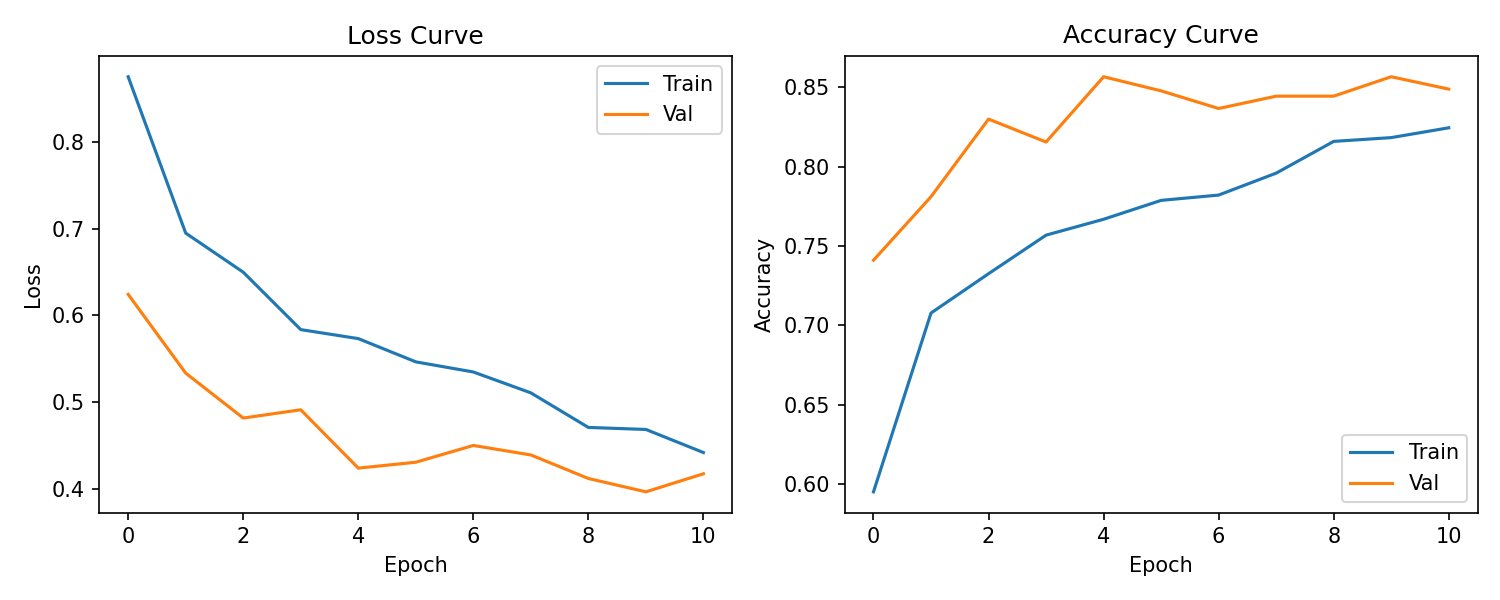
\includegraphics[width=\textwidth]{figures/baseline_cnn_curves.png}
  \vspace{-6mm}
  \caption{Baseline CNN (11 epochs, early stop).}
\end{subfigure}
\hfill
\begin{subfigure}[t]{0.48\textwidth}
  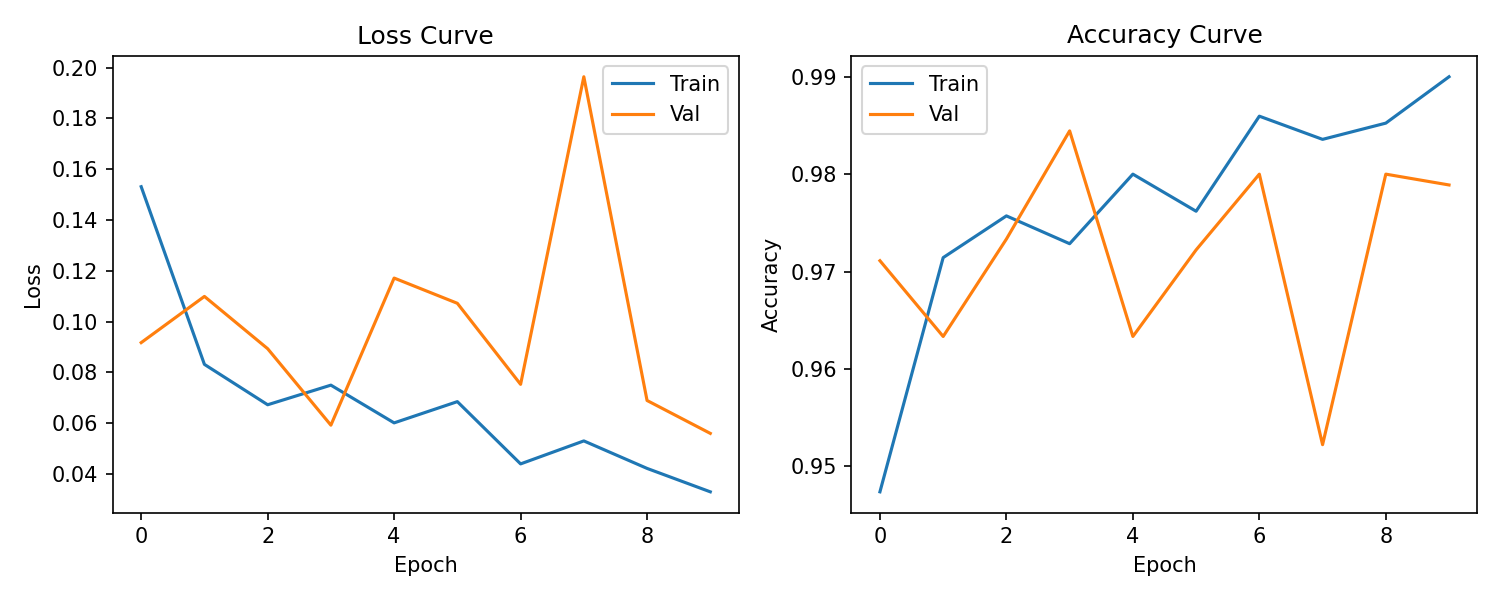
\includegraphics[width=\textwidth]{figures/resnet18_curves.png}
  \vspace{-6mm}
  \caption{ResNet-18 (10 epochs, early stop).}
\end{subfigure}
\vspace{-2mm}
\caption{Training and validation loss/accuracy curves for both classification models.}
\label{fig:curves}
\vspace{-4mm}
\end{figure}

\label{sec:lineart_results}
\textbf{Line art generation results.}
Initial training on Sketchy Database [5] sketches yielded Dice $>$0.97 but qualitatively blurry outputs (Figure~\ref{fig:sketchy}), because human sketches are not spatially aligned with photographs and U-Net requires pixel-level correspondence.
The high Dice reflected sparsity ($\sim$95\% white background), not meaningful line prediction.
After pivoting to edge-detection targets and introducing the weighted BCE + $L_1$ loss, retraining is in progress; early epochs already show sharper, category-appropriate outputs.

\begin{figure}[h]
\centering
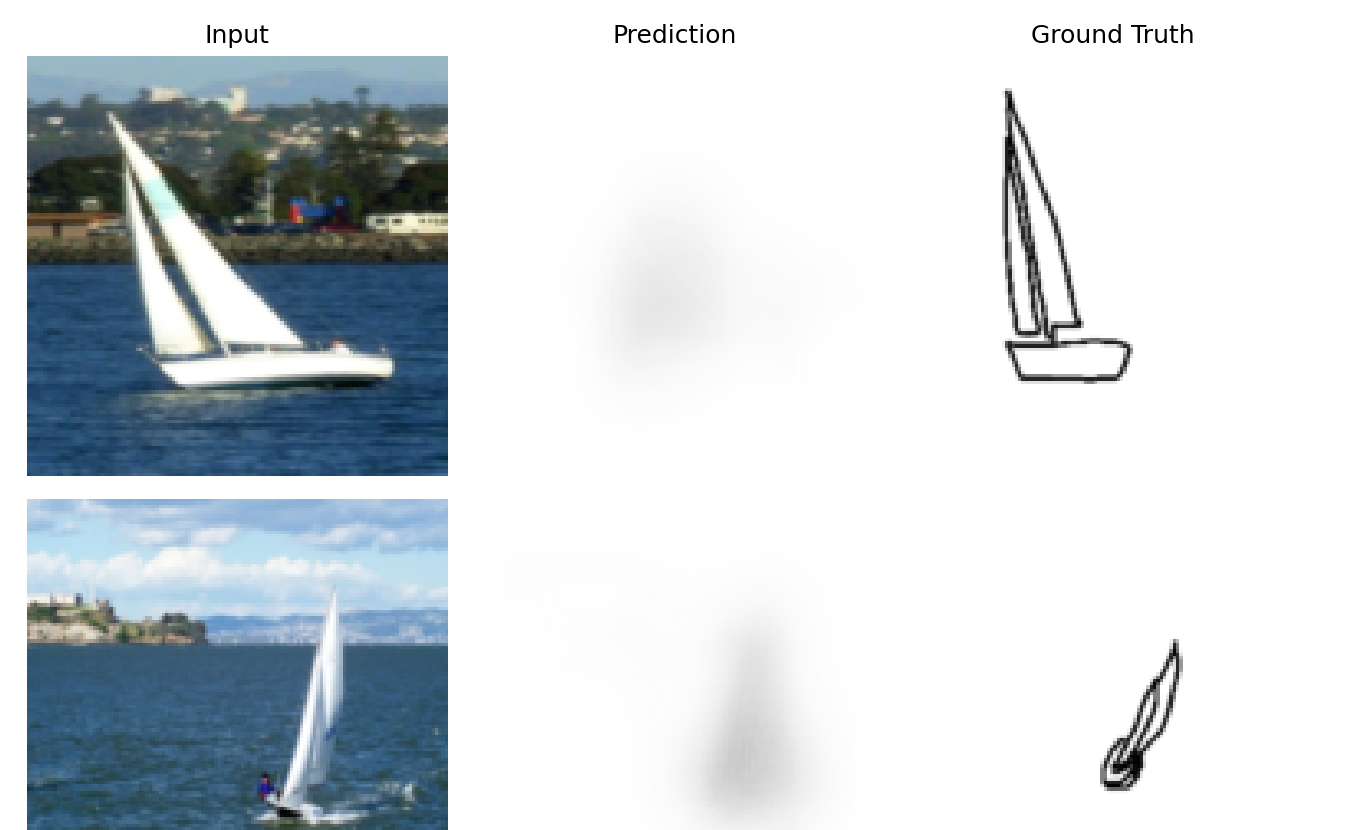
\includegraphics[width=0.65\textwidth]{figures/unet_vehicle_samples.png}
\vspace{-3mm}
\caption{Sketchy-trained U-Net: input (left), prediction (middle, blurry), ground truth sketch (right). Spatial misalignment causes regression-to-mean.}
\label{fig:sketchy}
\vspace{-4mm}
\end{figure}

\textbf{Feasibility \& next steps.}
Classification is solved (98.78\%). The current U-Net predictions produce only faint shadow-like blobs rather than crisp line strokes, because the Sketchy training targets are spatially misaligned with input photos; the model averages over all possible sketch poses and collapses to a gray silhouette.
This root cause has been identified and addressed: we have regenerated all targets using spatially-aligned edge detection and introduced weighted BCE to penalise missed lines.
Remaining: (1)~complete retraining with aligned targets to obtain clean line outputs; (2)~add perceptual loss [7] to encourage sharper strokes; (3)~blind evaluation on held-out photos.

% ============================================================
\begin{thebibliography}{9}
\small
\bibitem{1} O.~Ronneberger, P.~Fischer, T.~Brox. \textit{U-Net: Convolutional Networks for Biomedical Image Segmentation}. MICCAI, 2015.
\bibitem{2} J.~Canny. \textit{A Computational Approach to Edge Detection}. IEEE TPAMI, 8(6):679--698, 1986.
\bibitem{3} G.~Van Horn et al. \textit{Benchmarking Representation Learning for Natural World Image Collections}. CVPR, 2021.
\bibitem{4} B.~Zhou et al. \textit{Places: A 10 Million Image Database for Scene Recognition}. IEEE TPAMI, 40(6):1452--1464, 2018.
\bibitem{5} P.~Sangkloy et al. \textit{The Sketchy Database: Learning to Retrieve Badly Drawn Bunnies}. ACM TOG (SIGGRAPH), 35(4), 2016.
\bibitem{6} K.~He, X.~Zhang, S.~Ren, J.~Sun. \textit{Deep Residual Learning for Image Recognition}. CVPR, 2016.
\bibitem{7} M.~Li et al. \textit{Photo-Sketching: Inferring Contour Drawings from Images}. WACV, 2019.
\end{thebibliography}

\end{document}
